\documentclass[11pt]{article}
\usepackage[utf8]{inputenc}

%%% PAGE DIMENSIONS
\usepackage{geometry}
\geometry{a4paper}

\usepackage{graphicx}

%%% PACKAGES
\usepackage{booktabs}
\usepackage{paralist}
\usepackage{verbatim}
\usepackage{subfig}
\usepackage{chngcntr}
\usepackage{tikz}
\usepackage[colorlinks = true,
            linkcolor = black,
            urlcolor  = blue,
            citecolor = blue,
            anchorcolor = blue]{hyperref}
\usepackage[spanish]{cleveref}
\usepackage{placeins}

%%% HEADERS & FOOTERS
\usepackage{fancyhdr}
\pagestyle{fancy}
\renewcommand{\headrulewidth}{0pt}
\lhead{}\chead{}\rhead{}
\lfoot{}\cfoot{\thepage}\rfoot{}

%%% SECTION TITLE APPEARANCE
\usepackage{sectsty}
\allsectionsfont{\sffamily\mdseries\upshape}

%%% ToC (table of contents) APPEARANCE
\usepackage[nottoc,notlof,notlot]{tocbibind} % Put the bibliography in the ToC
\usepackage[titles,subfigure]{tocloft} % Alter the style of the Table of Contents
\renewcommand{\cftsecfont}{\rmfamily\mdseries\upshape}
\renewcommand{\cftsecpagefont}{\rmfamily\mdseries\upshape} % No bold!


\graphicspath{ {images/} }

\counterwithin*{figure}{section}
\counterwithin*{figure}{subsection}
\counterwithin*{figure}{subsubsection}

\counterwithin*{table}{section}
\counterwithin*{table}{subsection}
\counterwithin*{table}{subsubsection}

\addtolength{\cftfignumwidth}{2em}

\renewcommand{\thefigure}{
  \ifnum\value{subsection}=0
    \thesection.\arabic{figure}
  \else
    \ifnum\value{subsubsection}=0
      \thesubsection.\arabic{figure}
    \else
      \thesubsubsection.\arabic{figure}
    \fi
  \fi
}

\renewcommand{\thetable}{
  \ifnum\value{subsection}=0
    \thesection.\arabic{table}
  \else
    \ifnum\value{subsubsection}=0
      \thesubsection.\arabic{table}
    \else
      \thesubsubsection.\arabic{table}
    \fi
  \fi
}

%%% END Article customizations

%%% The "real" document content comes below...

\title{\Large Seguridad en Redes\\Practica 2.2}
\author{David Antuña Rodríguez\\Javier Carrión García}
\date{}

\begin{document}
  \raggedright

  \maketitle
  \newpage

  \section{OpenSSL}
    \subsection{Creacion de claves RSA, DSA, DH y EC}
      \par
      \textbf{Comandos}\\
      openssl genpkey -algorithm RSA -out rsakey.pem\\
      openssl pkey -pubout -in rsakey.pem -out rsapubkey.pem\\
      openssl pkey -in rsakey.pem -noout -text\\
      openssl pkey -pubin rsapubkey.pem -noout -text\\
      \vspace{2mm}
      openssl genpkey -genparam -algorithm DSA -out dsaparam.pem\\
      openssl genpkey -paramfile dsaparam.pem -out dsakey.pem\\
      openssl pkey -pubout -in dsakey.pem -out dsapubkey.pem\\
      openssl pkey -in dsakey.pem -noout -text\\
      openssl pkey -pubin dsapubkey.pem -nout -text\\
      \vspace{2mm}
      openssl genpkey -genparam -algorithm DH -out dhparam.pem\\
      openssl genpkey -paramfile dhparam.pem -out dhkey.pem\\
      openssl pkey -pubout -in dhkey.pem -out dhpubkey.pem\\
      openssl pkey -in dhkey.pem -noout -text\\
      openssl pkey -pubin dhpubkey.pem -nout -text\\
      \vspace{2mm}
      openssl genpkey -genparam -algorithm EC -out ecparam.pem\\
        \hspace{4mm}-pkeyopt ec\_paramgen\_curve:prime192v1\\
      openssl genpkey -paramfile ecparam.pem -out eckey.pem\\
      openssl pkey -pubout -in eckey.pem -out ecpubkey.pem\\
      openssl pkey -in eckey.pem -noout -text\\
      openssl pkey -pubin ecpubkey.pem -nout -text

      \bigskip
      \par
      RSA utiliza el teorema chino del resto para precomputar tres valores que aceleran el
      desencriptado del mensaje. Primero veamos cómo desencripta RSA.
      \begin{itemize}
        \item Sean \textbf{p} y \textbf{q} dos numeros primos diferentes escogidos aleatoriamente.
        \item Sea \textbf{n} la longitud de las claves rsa, privada y pública, \textit{n = pq}.
        \item Sea \textbf{d} $\equiv e^{-1}$ mod $\lambda$(n), donde e es un entero tal que 1 $<$
          e $<$ $\lambda$(n).
      \end{itemize}
      Sean m y c el mensaje desencriptado y encriptado, respectivamente.
      \begin{center}
        \Large
        \textit{m = $c^d$ mod n}
      \end{center}

      \par
      Dicho calculo puede resultar muy costoso debido al exponente, d, por lo que se aplica el
      teorema chino del resto para agilizarlo.

      \bigskip
      \par
      En primer lugar se precomputan $d_p$, $d_q$ y $q_{inv}$, con la precondición de que p $>$ q.
      \begin{itemize}
        \item $d_p$ = $e^{-1}$ mod (p-1)
        \item $d_q$ = $e^{-1}$ mod (q-1)
        \item $q_{inv}$ = $q^{-1}$ mod p
      \end{itemize}

      \par
      Una vez se poseen esos valores se pueden realizar los siguientes computos para desencriptar.
      \begin{itemize}
        \item $m_1$ = $c^{d_p}$ mod p
        \item $m_2$ = $c^{d_q}$ mod q
        \item $h$ = $q_{inv}$($m_1$ - $m_2$) mod p
      \end{itemize}

      \par
      Ahora el desencriptado no necesita resolver el exponente que incrementaba su coste.
      \begin{center}
        \Large
        \textit{m = $m_2$ + hq}
      \end{center}

    \subsection{Cifrado y descrifrado con RSA}
      \par
      \textbf{Comandos}\\
      openssl rand 32 -out keyfile\\
      openssl pkeyutl -encrypt -pubin -inkey rsapubkey.pem -in keyfile -out keyfile.bin\\
      openssl pkeyutl -decrypt -inkey rsakey.pem -in keyfile.bin $>$ keyfile2\\
      openssl enc -des3 -pass file:keyfile -in /etc/services -out cipher.bin\\
      openssl enc -d -des3 -pass file:keyfile2 -in cipher.bin


    \subsection{Firma y verificación con RSA, DSA y EC (ECDSA)}
      \par
      Para todas las firmas se ha empleado el algoritmo de hash sha256.

      \begin{figure}[!ht]
        \centering
        %\includegraphics[width = .6\textwidth]{sig_rsa}
        \caption{Firmado con rsa.}
      \end{figure}

      \begin{figure}[!ht]
        \centering
        %\includegraphics[width = .6\textwidth]{sig_dsa}
        \caption{Firmado con dsa.}
      \end{figure}

      \begin{figure}[!ht]
        \centering
        %\includegraphics[width = .6\textwidth]{sig_ec}
        \caption{Firmado con ec.}
      \end{figure}

      \par
      \textbf{Comandos}\\
      openssl dgst -sha256 -sign rsakey.pem -out sigrsa /etc/services\\
      openssl dgst -sha256 -verify pubkey.pem -signature sigrsa /etc/services\\
      \vspace{2mm}
      openssl dgst -sha256 -sign dsakey.pem -out sigdsa /etc/services\\
      openssl dgst -sha256 -verify pubkey.pem -signature sigdsa /etc/services\\
      \vspace{2mm}
      openssl dgst -sha256 -sign eckey.pem -out sigec /etc/services\\
      openssl dgst -sha256 -verify pubkey.pem -signature sigec /etc/services\\


    \subsection{Acuerdo de claves con DH y EC (ECDH)} \label{ecdh}
    \par
    \textbf{Comandos}\\
    openssl genpkey -paramfile dhparam.pem -out dhkey2.pem\\
    openssl pkey -pubout -in dhkey2.pem -out dhpubkey2.pem\\
    openssl pkey -in dhkey2.pem -noout -text\\
    openssl pkey -pubin dhpubkey2.pem -nout -text\\
    \vspace{2mm}
    openssl genpkey -paramfile ecparam.pem -out eckey2.pem\\
    openssl pkey -pubout -in eckey2.pem -out ecpubkey2.pem\\
    openssl pkey -in eckey2.pem -noout -text\\
    openssl pkey -pubin ecpubkey2.pem -nout -text\\
    \vspace{2mm}
    openssl pkeyutl -derive -inkey dhkey.pem -peerkey dhpubkey2.pem -out secret1dh\\
    openssl pkeyult -derive -inkey dhkey2.pem -peerkey dhpubkey.pem -out secret2dh\\
    cmp secret1dh secret2dh\\
    xxd secret1dh\\
    xxd secret2dh\\
    \vspace{2mm}
    openssl pkeyutl -derive -inkey eckey.pem -peerkey ecpubkey2.pem -out secret1ec\\
    openssl pkeyult -derive -inkey eckey2.pem -peerkey ecpubkey.pem -out secret2ec\\
    cmp secret1ec secret2ec\\
    xxd secret1ec\\
    xxd secret2ec

  \section{GnuPG}
    \subsection{Creación y gestión de claves PGP}
      \begin{figure}[!ht]
        \centering
        %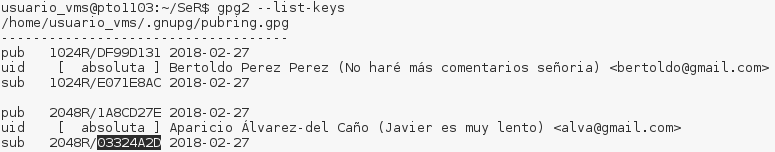
\includegraphics[width = .6\textwidth]{sring}
        \caption{Claves públicas del anillo.}
      \end{figure}

      \begin{figure}[!ht]
        \centering
        %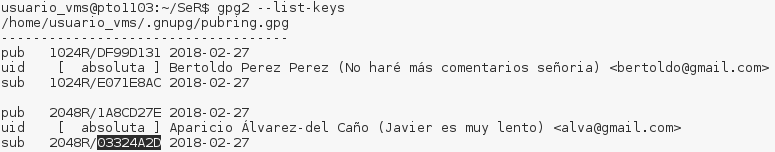
\includegraphics[width = .6\textwidth]{sring}
        \caption{Claves públicas del anillo tras importar.}
      \end{figure}

      \par
      \textbf{Comandos}\\
      gpg2 $--$list-keys \hspace{10mm} Hacer captura(sring)\\
      \vspace{2mm}
      gpg2 $--$gen-key \hspace{10mm} Usar dos veces para crear dos claves, contraseña: seguridad\\
      gpg2 $--$output keys.gpg -a $--$export id \hspace{10mm} Listar las keys y coger el id de una de las creadas\\
      \vspace{2mm}
      gpg2 $--$import pubInma.gpg\\
      gpg2 $--$list-keys \hspace{10mm} Hacer captura(nring)\\

    \subsection{Cifrado y descifrado}
      \par
      Hemos cifrado el fichero con la clave pública que has subido al campus.

      \par
      \textbf{Comandos}\\
      cp /etc/services \$HOME/SeR/services\\
      gpg2 --output services.gpg $--$encrypt $--$recipient (id de la clave de inma) -a services

    \subsection{Firma y verificación}
      \par
      \textbf{Comandos}\\
      gpg2 $--$list-keys\\
      Probar para dos claves, una de ellas ha de ser la que hemos exportado para subir\\
      \vspace{2mm}
      gpg2 $--$sign --output sign(id1) -u (id1) -a $--$digest-algo md5 /etc/services\\
      gpg2 $--$verify sign(id1)\\
      \vspace{2mm}
      gpg2 $--$sign --output sign(id2) -u (id2) -a $--$digest-algo sha256 /etc/services\\
      gpg2 $--$verify sign(id2)\\
\end{document}
